\section{Método de diseño}
Según el capítulo 9 de la norma E-060 la resistencia de diseño de todos los elementos debe ser por lo menos la resistencia requerida según:
\begin{equation}
   \phi R_{n}\geqslant R_{u} 
\end{equation}
\myequations{Requisito de resistencia según E-060}
\vspace{-1.4cm}
\section{Combinaciones de diseño}
Según el capitulo 9 de la \cite{E-060} las combinaciones de diseño serán:
    \begin{align}
       &U=1.4\;CM+1.7\;CV\myequations{Combinaciones de carga gravitacional} \\
        &U=1.25\left ( CM+CV \right )\pm CS\myequations{Combinaciones con carga sísmica 1}\\
        &U=0.9\;CM+CV \pm CS \myequations{Combinaciones con carga sísmica 2}        
    \end{align}

\newpage
\noindent
Donde:\\
$CM$: Carga Muerta\\
$CV$: Carga viva\\
$CS$: Carga de sismo, según la \cite{E-030} en el artículo 21.1 el análisis se puede realizar considerando que el total de la fuerza sísmica actúa independiente en cada dirección ortogonal, por lo que se tienen 5 combinaciones independientes considerando el sismo en cada dirección.
\section{Diseño de elementos estructurales}
\subsection{Diseño de vigas}
\subsubsection{Factores de minoración}
% Table generated by Excel2LaTeX from sheet 'Hoja1'
\begin{table}[ht!]
  \centering
  \caption{Factores de minoración para el diseño de vigas}
        {
\extrarowheight = 0ex
\renewcommand{\arraystretch}{1.15}
    \begin{tabular}{|>{\centering\arraybackslash}m{2.8cm}|>{\centering\arraybackslash}m{3.8cm}|>{\centering\arraybackslash}m{3.8cm}|}
    \hline
    \textbf{Articulo de E-060} & \textbf{Solicitación} & \textbf{Factor de minoración} \\
    \hline
    9.2.3.1   & Flexión & $\phi_{f}$=0.90 \\
    \hline
    9.3.2.3   & Corte y torsión & $\phi_{c}$=0.85 \\
    \hline
    \end{tabular}%
    }
    \caption*{\small Fuente: \it \cite{E-060}}
  \label{tab:addlabel}%
\end{table}%
\vspace{-0.8cm}
\subsubsection{Diseño a flexión}
\begin{figure}[h!]
    \centering
    \caption{Análisis de una viga simplemente armada}
    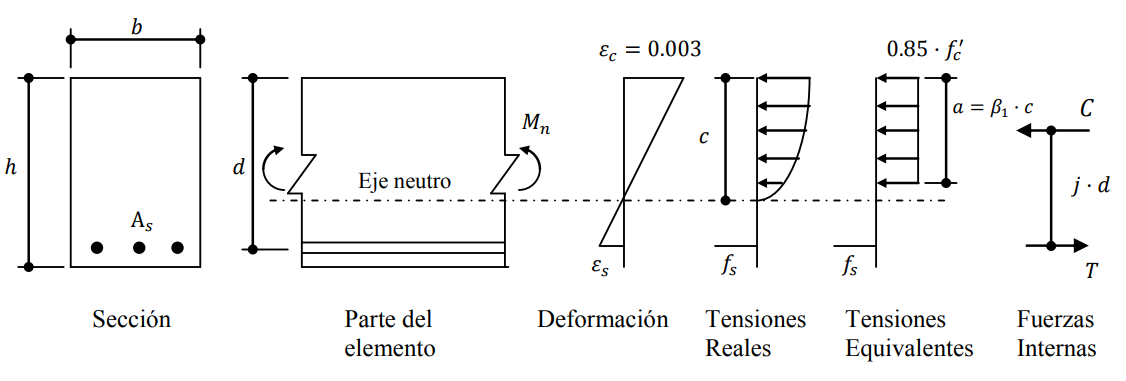
\includegraphics[scale=0.67]{IMAGENES/d9.PNG}
    \caption*{\small Fuente: \it \cite{cordova2015}}
    \label{vig}
\end{figure}
\begin{theo}[Art. 10.2.7.1 y 10.2.7.3 E-060 :]{thm:ca1}
Un  esfuerzo  en  el  concreto  de  0,85  f’c uniformemente  distribuido  en  una  zona  de compresión equivalente, limitada por los bordes de la sección transversal del elemento y por una línea recta paralela al eje neutro, a una distancia a = $\beta$c de la fibra de deformación unitaria máxima en compresión.\\
Para f’c entre 17 y 28 MPa, el factor $\beta$1 se debe tomar como 0,85.   Para f’c mayor o igual a 56 MPa,  $\beta$1 se debe tomar como 0,65.  Para f’c entre 28 y 56 MPa se debe interpolar linealmente entre 0,85 y 0,65.
\end{theo}
\noindent
%\vspace{-1cm}
Considerando que el acero de refuerzo alcanza la fluencia y los esfuerzos del concreto se representan mediante el bloque de compresión equivalente según la figura \ref{vig} y la \cite{E-060}:
\begin{flalign}
&\textup{Tracción en el acero de refuerzo:}&T&=A_{s}\cdot f_{y}&\\
&\textup{Compresión en el concreto:}&C&=0.85\cdot f_{c}^{'}\cdot a\cdot b&\\
&\textup{Brazo del par de fuerzas:}&j&=d-\frac{a}{2}&\\
&\textup{Momento resistente:}&\phi\cdot M_{n}&=\phi\cdot A_{s}\cdot f_{y}\left ( d-\frac{a}{2} \right )\label{15}&
\end{flalign}
\noindent
Haciendo uso de la ecuación de equilibrio $T&=C$ se puede llegar a la ecuación  (\ref{16}), y combinándola con (\ref{15}) haciendo uso de $M_{u}=\phi M_{n}$ se puede llegar a la expresión (\ref{ace}) para calcular el acero de refuerzo en una viga ignorando el refuerzo en compresión para un momento ultimo dado $M_{u}$.
\begin{gather}
%M_{u}&=\phi\cdot A_{s}\cdot f_{y}\left ( d-\frac{a}{2} \right )\label{15}&\\
a=\frac{A_{s}\cdot f_{y}}{0.85\cdot f_{c}^{'}\cdot b}\label{16}\\
A_{s}=\frac{0.85\;f_{c}^{'}\;b\;d}{f_{y}}\left ( 1-\sqrt{1-\frac{2\;M_{u}}{\phi\;0.85\;f_{c}^{'}\;b\;d^{2} }} \right )
\label{ace}
\end{gather}
\newpage
\noindent En la figura \ref{vigm} se muestra que la viga del eje 6 es la que presenta mayor solicitación de momento para la condición de envolvente de las combinación de diseño con las fuerzas sísmicas escaladas. A continuación se muestra el diseño del elemento mencionado.
\begin{figure}[h!]
    \centering
    \caption{Viga con mayor solicitación}
    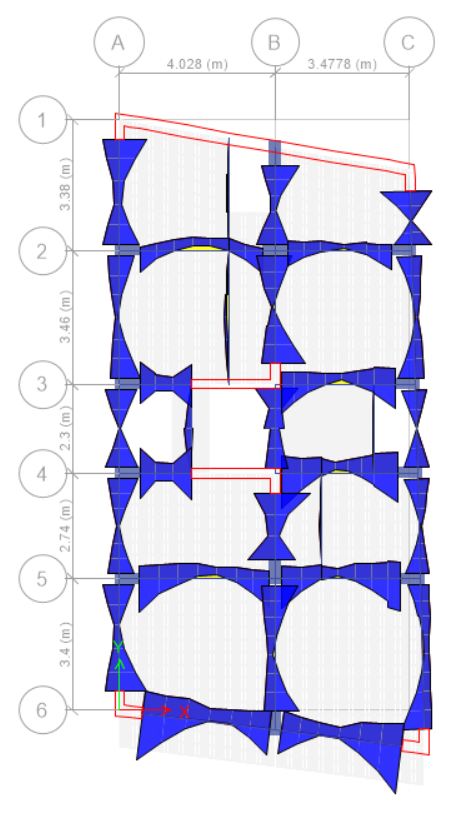
\includegraphics[scale=0.8]{IMAGENES/d10.PNG}
    %\caption*{\small Fuente: \it \cite{cordova2015}}
    \label{vigm}
\end{figure}

\newpage
\begin{figure}[h!]
    \centering
    \begin{tikzpicture}
        \tikzset{
        hatch distance/.store in=\hatchdistance,
        hatch distance=10pt,
        hatch thickness/.store in=\hatchthickness,
        hatch thickness=2pt
    }

    \makeatletter
    \pgfdeclarepatternformonly[\hatchdistance,\hatchthickness]{flexible hatch}
    {\pgfqpoint{0pt}{0pt}}
    {\pgfqpoint{\hatchdistance}{\hatchdistance}}
    {\pgfpoint{\hatchdistance-1pt}{\hatchdistance-1pt}}%
    {
        \pgfsetcolor{\tikz@pattern@color}
        \pgfsetlinewidth{\hatchthickness}
        \pgfpathmoveto{\pgfqpoint{0pt}{0pt}}
        \pgfpathlineto{\pgfqpoint{0pt}{\hatchdistance}}
        %\pgfpathlineto{\pgfqpoint{\hatchdistance}{\hatchdistance}}
        \pgfusepath{stroke}
    }
    \begin{axis}
    [grid=both,
    grid style={line width=.1pt,dashed, draw=gray!10},
    major grid style={line width=.2pt,draw=gray!50},name=plot, xlabel={$x$ (m)},ylabel={$M_{u}$ (ton.m)},xmin=0.15,xmax=3.3,
    ymin=-6,ymax=10,width=.85\textwidth,height=8cm,xtick distance=0.4,ytick distance=3]
    \addplot[name path = A,OrangeRed,ultra thick]
    table{DATOS/env.txt};\label{xx}
    \addplot[name path = B,MidnightBlue,ultra thick] table{DATOS/env2.txt};\label{yy}
    %\addplot[MidnightBlue,ultra thick,mark=o] table{DATOS/DYY.txt};\label{yy}
    %\addplot[black,mark=triangle*] table{./espectro R=8.txt};\label{f}
    %\addplot[red,mark=o] table{./data/generator.txt};\label{g}
    %\addplot[blue] table{./data/simulated_total.txt};\label{s}
    %\addplot[green,dashed] table{./data/theoretical_total.txt};\label{t}
   % \tikzfillbetween[of=A and B]{pattern=flexible hatch};
    \addplot[pattern=flexible hatch,
        hatch distance=7pt,hatch thickness=0.5pt,
        pattern color=cyan] fill between [of=A and B];
    \end{axis}
    \end{tikzpicture}
    \caption{Diagrama de momento flector viga EJE 6 tramo B-C (Envolvente)}
    \label{der}
\end{figure}
\noindent 

Geometría de la viga:
\FPset\h{50} 
\FPset\bv{30} 
\FPset\ln{3.15} 
\FPeval{\defe}{round(\h-6,0)}
\begin{itemize}
  \item Ancho: $b=30 \mathrm{~cm}$

  \item Peralte: $h=\h \mathrm{~cm}$

  \item Peralte efectivo: $d=h-6 \mathrm{~cm}\footnote{\cite{pasino2011} recomienda estimar el peralte efectivo como $d=h-6$ y $d=h-9$ para 1 y 2 capas de acero respectivamente}=\h-6=\defe \mathrm{~cm}$ 

  \item Luz libre: $l_{n}=\ln \mathrm{~m}$
  
\end{itemize}

Datos de los materiales:

Concreto:

\begin{itemize}
  \item Resistencia a la compresión: $\displaystyle f_{c}^{\prime}=210 \;\frac{\mathrm{kg}}{\mathrm{cm}^{2}}$

  \item Deformación unitaria del concreto: $\varepsilon_{c}=0,003$

  \item Densidad del concreto: $\displaystyle\gamma_{c}=2,40\;\frac{\mathrm{ ton }}{\mathrm{m}^{3}}$

\end{itemize}
\newpage
Acero de refuerzo:

\begin{itemize}
  \item Esfuerzo de fluencia: $\displaystyle f_{y}=4200\; \frac{\mathrm{kg}}{\mathrm{cm}^{2}}$

  \item Módulo de elasticidad: $\displaystyle E_{\mathrm{s}}=2 \cdot 10^{6} \;\frac{\mathrm{kg}}{\mathrm{cm}^{2}}$

  \item Deformación de fluencia: $\displaystyle \varepsilon_{s}=\frac{f_{y}}{E_{s}}=\frac{4200}{2 \cdot 10^{6}}=0,0021$

\end{itemize}
\noindent Aplicando la ecuación \ref{ace} se obtiene que se requiere para el extremo izquierdo $3.17\;{\mathrm{cm}^{2}}$ y $2.54\;{\mathrm{cm}^{2}}$ superior e inferior respectivamente y para el extremo derecho $6.19\;{\mathrm{cm}^{2}}$ y $3.17\;{\mathrm{cm}^{2}}$.\\
Por lo que se coloca $2 \phi 5 / 8"=3.96 \mathrm{~cm}^{2}$ como acero corrido superior e inferior y en el extremo superior derecho se coloca como bastón $2 \phi 5 / 8$" haciendo un total de $4 \phi 5 / 8"=7.92 \mathrm{~cm}^{2}$.\\
\textit{Verificación del espaciamiento entre barras}\\
Según el articulo 7.6.2 y 3.3.2 la distancia libre entre barras paralelas de una capa debe ser el mayor de:
\begin{enumerate}
\item[] (a): $d_{b}$ Diámetro de la varilla longitudinal
\item[] (b): $25 \mathrm{~mm}$
\item[] (c): $4/3$ del tamaño máximo del agregado
\end{enumerate}

\begin{figure}[h!]
    \centering
    \caption{Requisitos de colocación del refuerzo}
    \subfigure[Espaciamiento mínimo entre barras]{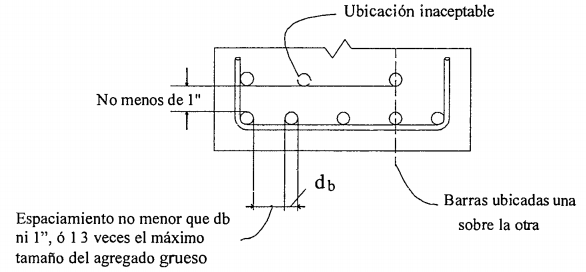
\includegraphics[height=45mm]{IMAGENES/sep.PNG}}\hspace{5mm}
    \subfigure[Recubrimiento]{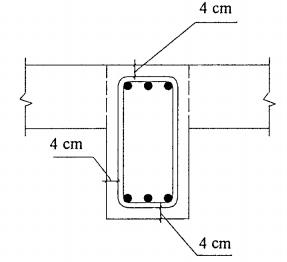
\includegraphics[height=45mm]{IMAGENES/rec.PNG}}
    \caption*{\small Fuente: \it \cite{pasino2011}}
    \label{3}
\end{figure}
Según el articulo 7.7.1 el recubrimiento mínimo para vigas de concreto construidos en sitio sin exposición a la intemperie ni al contacto con el suelo es de 4cm.

La separación entre barras donde existen $4 \phi 5 / 8"$ considerando estribos de 3/8" de diámetro ($d_{e}$) el peralte efectivo sera::
\FPset\rec{4}
\FPset\numvar{4}
\FPeval{\estcm}{round(3*2.54/8,2)}
\FPeval{\vacm}{round(5*2.54/8,2)}
\FPeval{\smin}{round((\bv-2*\rec-2*\estcm-\numvar*\vacm)/(\numvar-1),2)}
\begin{flalign}
s_{var}&=\frac{b-2\cdot r_{e}-2\cdot d_{e}-n_{v}\cdot d_{b}}{n_{v}-1}\\
s_{var}&=\frac{\bv-2\cdot \rec-2\cdot\estcm-\numvar\cdot \vacm}{\numvar-1}=\smin\mathrm{~cm}\notag
\end{flalign}
\textit{Peralte efectivo}
\FPeval{\deft}{round(\h-\rec-\estcm-\vacm/2,2)}
\begin{flalign}
d_{efe}&=h-r_{e}-d_{e}-d_{b}/2\\
d_{efe}&=\h-\rec-\estcm-\vacm/2=\deft\mathrm{~cm}\notag
\end{flalign}
La altura del bloque en compresión y el momento resistente del acero corrido sera:
\FPset\ascor{3.96}
\FPset\asder{7.92}
\FPset\fc{210}
\FPset\fy{4200}
\FPeval{\acor}{round((\fy*\ascor)/(0.85*\fc*\bv),2)}
\FPeval{\mncor}{round((0.9*\fy*\ascor)*(\defe-\acor/2)/100000,2)}
\begin{align*}
a&=\frac{A_{s}\cdot f_{y}}{0.85\cdot f_{c}^{'}\cdot b}\\
a&=\frac{\ascor\cdot \fy}{0.85\cdot\fc\cdot\bv}=\acor\;\mathrm{~cm}\\
\phi M_{n}&=\phi\cdot A_{s}\cdot f_{y}\left ( d-\frac{a}{2} \right )\\
\phi M_{n,1}&=0.9\cdot \ascor \cdot \fy\left ( \defe-\frac{\acor}{2} \right )=\mncor\;\mathrm{~ton.m} 
\end{align*}
\FPeval{\ader}{round((\fy*\asder)/(0.85*\fc*\bv),2)}
\FPeval{\mnder}{round((0.9*\fy*\asder)*(\defe-\ader/2)/100000,2)}
Similarmente en el extremo superior derecho:
\begin{align*}
%a&=\frac{A_{s}\cdot f_{y}}{0.85\cdot f_{c}^{'}\cdot b}\\
a&=\frac{\asder\cdot \fy}{0.85\cdot\fc\cdot\bv}=\ader\;\mathrm{~cm}\\
%\phi M_{n}&=\phi\cdot A_{s}\cdot f_{y}\left ( d-\frac{a}{2} \right )\\
\phi M_{n,2}&=0.9\cdot \asder \cdot \fy\left ( \defe-\frac{\ader}{2} \right )=\mnder\;\mathrm{~ton.m} 
\end{align*}
\newpage

\subsubsection{Desarrollo del refuerzo para flexión Art. 12.10}
%\newpage
\begin{theo}[Art. 12.10.3 :]{thm:ca1}
El refuerzo se debe extender, más allá del punto en el que ya no es necesario para resistir flexión, una distancia igual a d ó 12 db, la que sea mayor, excepto en los apoyos de vigas simplemente apoyadas y en el extremo libre de los voladizos.
\end{theo}
\noindent
Donde:\\
$d_{b}$ : Diámetro de la varilla\\
$d$ : Peralte efectivo\\

\begin{figure}[h!]
    \centering
    \caption{Punto teórico de corte}
    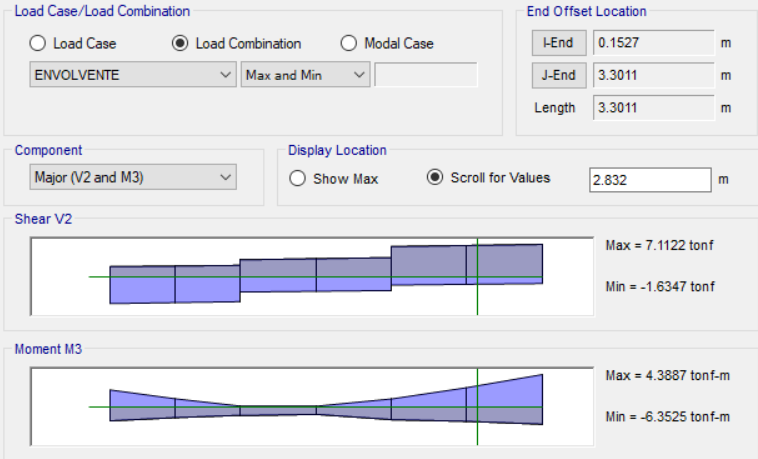
\includegraphics[scale=0.7]{IMAGENES/pcor.PNG}
    %\caption*{\small Fuente: \it \cite{cordova2015}}
    \label{vigcor}
\end{figure}

\begin{figure}[h!]
    \centering
    \caption{Corte de acero}
    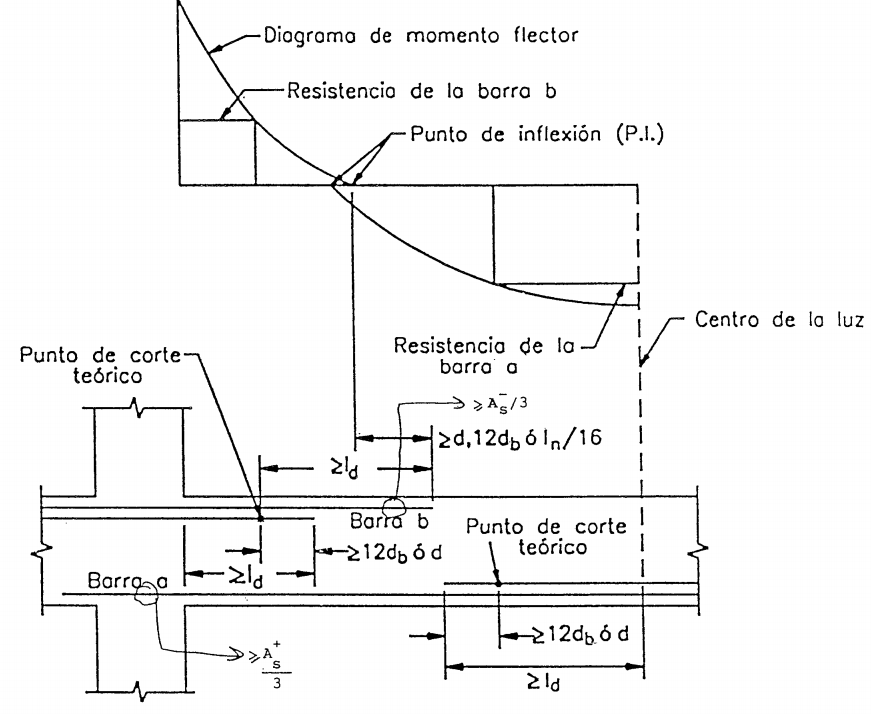
\includegraphics[scale=0.6]{IMAGENES/corte.PNG}
    \caption*{\small Fuente: \it \cite{pasino2011}}
    \label{vigm}
\end{figure}

\noindent La mayor dimensión entre d y 12 db resulta d=44 cm. Como se aprecia en la figura \ref{vigcor} la longitud teórica de corte sera: 3.3011m - 2.832m=0.469m, la longitud del bastón sera: 46.9cm+44cm $\approx$ 100cm.
\newpage
\begin{theo}[Art. 12.1 :]{thm:ca1}
La tracción o compresión calculada en el refuerzo en cada sección de los elementos de concreto estructural, debe ser desarrollada hacia cada lado de dicha sección mediante una longitud embebida en el concreto (longitud de anclaje), gancho, dispositivo mecánico o una combinación de ellos. Los ganchos no se deben emplear para el anclaje de barras en compresión.
\end{theo}
\noindent
Según la tabla 12.1 de la \cite{E-060} la longitud de desarrollo se calcula con la ecuación \ref{ld}
\begin{align}
l_{d}=\left(\frac{f_{y} \cdot \psi_{t} \cdot \psi_{e} \cdot \lambda}{8,2 \cdot \sqrt{f_{c}^{\prime}}}\right) d_{b}
\label{ld}
\end{align}
\noindent
Donde:\\
$\psi_{t}=1,3$ Para varillas superiores\\
$\psi_{e}=1,0$ Para varillas sin tratamiento superficial\\
$\lambda=1,0$ Para concretos de peso normal
\FProot\rc{\fc}{2}
\FPeval{\dbcm}{round(5*2.54/8,2)}
\FPeval{\ld}{round(\fy*1.3*\dbcm/(8.2*\rc),2)}
\begin{align*}
l_{d}=\left(\frac{\fy \cdot 1.3 \cdot 1\cdot 1}{8,2 \cdot \sqrt{\fc}}\right) \dbcm=\ld\;\mathrm{~cm}\approx\;75\;\mathrm{~cm}
%\label{ld}
\end{align*}
\noindent El bastón adicional consiste en 2 varillas de 5/8", el punto de corte de la primera varilla según lo calculado fue de 100cm, para la segunda varilla se puede proceder de manera similar calculando el momento que resiste 3 varillas de 5/8", sin embargo debe ser por lo menos 75cm para que pueda desarrollar. El esquema final de armado se puede ver en la figura.
\begin{figure}[h!]
    \centering
    \caption{Demanda y capacidad de la viga}
    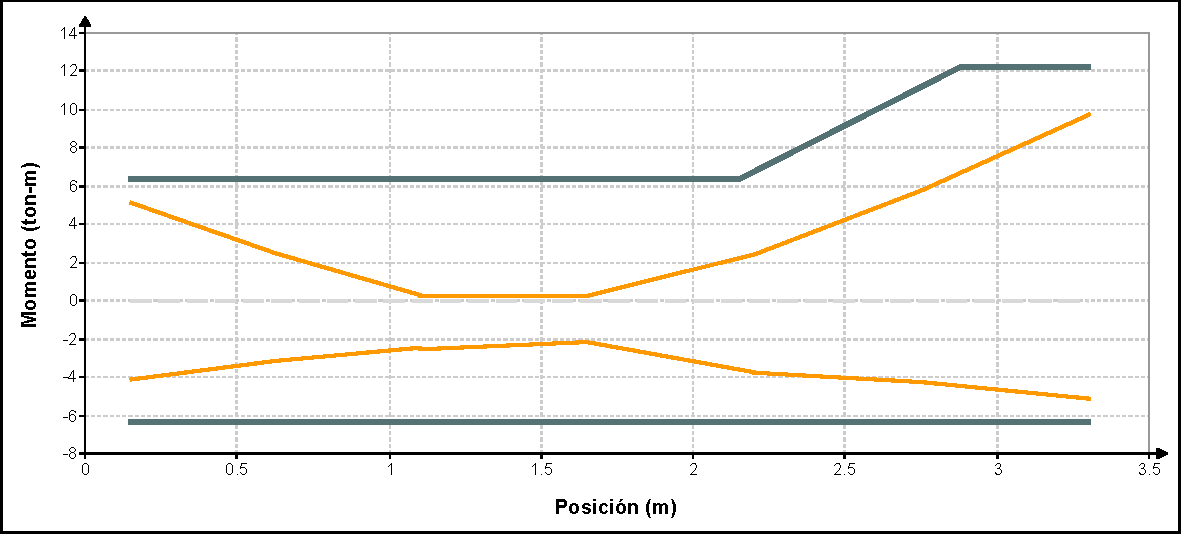
\includegraphics[scale=0.6]{IMAGENES/capb.pdf}
    %\caption*{\small Fuente: \it \cite{cordova2015}}
    \label{vigm}
\end{figure}

\textit{Desarrollo de ganchos estándar en tracción}
\begin{theo}[Art. 12.5.1 y 12.5.2 :]{thm:ca1}
La longitud de desarrollo para barras corrugadas en tracción que terminen en un gancho estándar (véase 7.1), se debe calcular según 12.5.2 y los factores de modificación de 12.5.3, pero no debe ser menor que el menor valor entre  8 db  y 150 mm.\\
Para las barras corrugadas, $l_{dg} $ se calcula con $\psi_{e}$ igual a 1,2 
para refuerzo con recubrimiento epóxico y $\lambda$ igual a 1,3 para concretos livianos.  Para otros casos, $\psi_{e}$  y $\lambda$  deben tomarse igual a 1,0
\end{theo}
\FPeval{\ldg}{round(\fy*0.075*\dbcm/(\rc),2)}
\begin{flalign}
l_{dg}&=\left (0.075 \cdot \psi_{e}\cdot \lambda\cdot  f_{y}/\sqrt{f_{c}^{'}} \right )d_{b}\\
l_{dg}&=\left (0.075 \cdot 1.00 \cdot 1.00 \cdot  \fy/\sqrt{\fc} \right )\dbcm=\ldg\mathrm{~cm}\notag
\end{flalign}
\noindent Se concluye que se necesita por lo menos 40cm para que el acero de 5/8" desarrolle con gancho estándar, dado que la viga del eje 6 llega a columnas con peraltes de 55cm se asegura el anclaje sin necesidad de alguna consideración especial como se menciona en 12.5.3.
\begin{figure}[h!]
    \centering
    \caption{desarrollo de gancho estándar}
    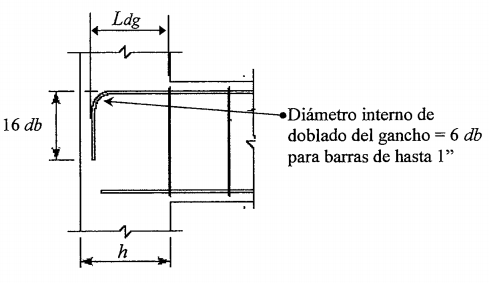
\includegraphics[scale=1]{IMAGENES/gancho.PNG}
    \caption*{\small Fuente: \it \cite{pasino2011}}
    \label{vigm}
\end{figure}
\subsubsection{Refuerzo mínimo de elementos sujetos a flexión Art. 10.5}
\begin{theo}[Art. 10.5.1 E-060 :]{thm:ca1}
En cualquier sección de un elemento estructural - excepto en zapatas y losas macizas - sometidos a flexión, donde por el análisis se requiere refuerzo de acero en tracción, el área de acero que se proporcione será la necesaria para que la resistencia de diseño de la sección sea por lo menos 1.2 veces el momento de agrietamiento de la sección bruta $M_{cr}$ $\left ( \phi\;M_{n}\geq1.2\;M_{cr} \right )$.
\end{theo}
\vspace{-0.8cm}
\begin{flalign}
\textup{Ecu.(9.12) E-060:}\hspace{4.3cm} f_{r}=2\sqrt{f_{c}^{'}}&&
\end{flalign}
\myequations{Modulo de ruptura del concreto}
\vspace{-1.5cm}
\begin{flalign}
\textup{Ecu.(9.11) E-060:}\hspace{4.3cm} M_{cr}=\frac{f_{r}\cdot I_{g}}{Y_{t}}&&
\end{flalign}
\myequations{Momento de agrietamiento}
\vspace{-0.8cm}
\noindent La norma el articulo 10.5.2 también menciona que el acero mínimo en secciones rectangulares no debe ser menor que la ecuación \eqref{min}, \cite{pasino2011} menciona que lo anterior implica que el momento resistente es aproximadamente 1.5 veces el momento de agrietamiento por lo que se cumple con lo dispuesto en 10.5.
\begin{flalign}
\textup{Ecu.(10.3) E-060:}\hspace{3.6cm}A_{s}=\frac{0.7\sqrt{f_{c}^{'}}}{f_{y}}\cdot b_{w}\cdot d&&\label{min}
\end{flalign}
\FPeval{\rb}{round((0.7*\rc*\bv*\defe)/\fy,2)}
\FPeval{\pmin}{round((0.7*\rc)/\fy,4)}
\begin{equation*}
A_{s}=\frac{0.7\sqrt{\fc}}{\fy}\cdot \bv\cdot \defe=\pmin\cdot \bv\cdot \defe=\rb\;\mathrm{cm}^{2}
\end{equation*}
%$\centering \displaystyle A_{s}=\frac{0.7\sqrt{\fc}}{\fy}\cdot \bv\cdot \defe=\rb\;\mathrm{cm}^{2}$\\

%\begin{theo}[Art. 10.5.3 E-060 :]{thm:ca1}
    %No es necesario satisfacer los requisitos de 10.5.1 y 10.5.2, si en cada sección del elemento el área de acero en tracción proporcionada es al menos un tercio superior a la requerida por análisis.
%\end{theo}
\noindent
El acero colocado es mayor al mínimo dispuesto por la norma.
\subsubsection{Refuerzo máximo de elementos sujetos a flexión}
\begin{theo}[Art. 10.3.4 E-060 :]{thm:ca1}
En elementos no preesforzados sujetos a flexión o flexocompresión en los cuales $\phi P_{n}$ sea menor que 0,1 f’c Ag, el refuerzo de acero en tracción no deberá exceder de 0,75 Asb, donde Asb es la cantidad de acero en tracción que produce la falla balanceada en la sección, definida en 10.3.2.
\end{theo}

\begin{theo}[Cuantía balanceada Art. 10.3.2 E-060 :]{thm:ca1}
La condición de falla balanceada se produce en una sección transversal cuando el refuerzo en tracción alcanza la deformación unitaria correspondiente a fy al mismo tiempo que el concreto en compresión alcanza su deformación unitaria máxima utilizable de 0.003. Este criterio es general y se aplica a secciones de cualquier forma sin acero en compresión o con él.
\end{theo}
\begin{align}
\rho_{b}&=\frac{0,85 \cdot f_{c}^{\prime} \cdot \beta_{1}}{f_{y}}\left(\frac{\varepsilon_{c}}{\varepsilon_{y}+\varepsilon_{c}}\right)\\
\rho_{\max }&=0,75\;\rho_{b}
%\label{max}
\end{align}
\begin{figure}[h!]
    \centering
    \caption{Cuantía balanceada}
    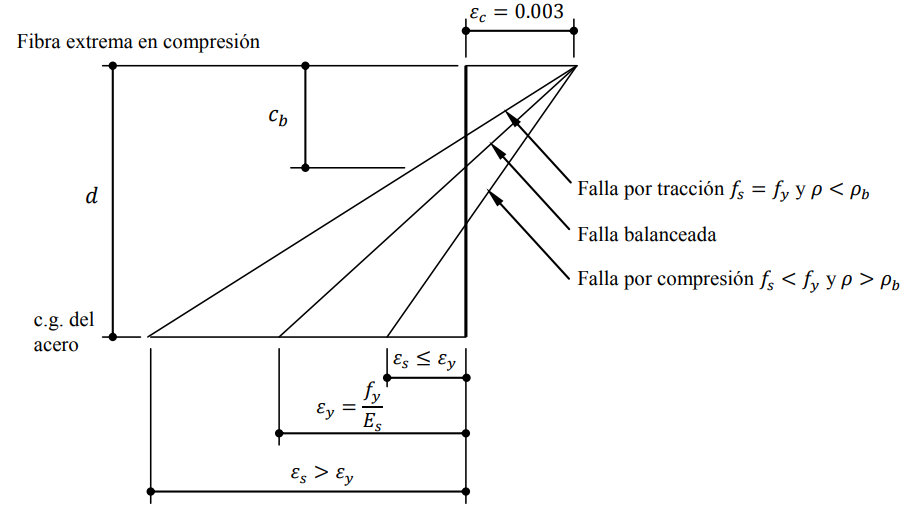
\includegraphics[scale=0.6]{IMAGENES/d1.PNG}
    \caption*{\small Fuente: \it \cite{cordova2015}}
    \label{ver}
\end{figure}
\FPeval{\rcc}{round((0.85*\fc*0.85*0.003)/(\fy*(0.003+0.0021)),4)}
\FPeval{\rcd}{round(0.75*\rcc,3)}
\newpage
\noindent
Para $f_{c}^{\prime}=210\;\mathrm{cm}^{2}$ y $f_{y}=4200\;\mathrm{cm}^{2}$ la cuantía balanceada y máxima sera:
\begin{gather*}
\rho_{b}=\frac{0,85 \cdot \fc \cdot 0.85}{\fy}\left(\frac{0.003}{0.0021+0.003}\right)=\rcc\\
\rho_{\max }=0,75\cdot\rcc=\rcd
%\label{max}
\end{gather*}
\noindent La cuantía colocada esta muy por debajo de la máxima dispuesta por la norma.
%\newpage
\subsubsection{Disposición del acero del refuerzo longitudinal (Art. 21.4.4 y 25.5.2)}
\begin{theo}[Art. 21.4.4.1 y 21.5.2.1 :]{thm:ca1}
\textit{Vigas en sistemas de muros}\\
Deberá existir refuerzo continuo a todo lo largo de la viga, constituido por dos barras tanto en la cara superior como en la inferior, con un área de acero no menor de la especificada en 10.5. No se aplicará lo dispuesto en 10.5.3.\\
\textit{Vigas de sistemas duales o pórticos}\\
Adicionalmente a lo anterior la cuantía de refuerzo en tracción no deberá exceder de 0,025.
\end{theo}
\begin{theo}[Art. 21.4.4.3 y 21.5.2.2 :]{thm:ca1}
La resistencia a momento negativo y positivo en cualquier sección a lo largo de la longitud del elemento deben ser mayores de un cuarto de la máxima resistencia a momento proporcionada en la cara de cualquiera de los nudos.\\
\textit{Vigas en sistemas de muros}\\
La resistencia a momento positivo en la cara del nudo no debe ser menor que un tercio de la resistencia a momento negativo provista en dicha cara.\\
\textit{Vigas de sistemas duales o pórticos}\\
La resistencia a momento positivo en la cara del nudo no debe ser menor que la mitad de la resistencia a momento negativo provista en dicha cara.
\end{theo}

\begin{figure}[h!]
    \centering
    \caption{Requisitos del refuerzo longitudinal en vigas}
    \subfigure[Sistemas de muros]{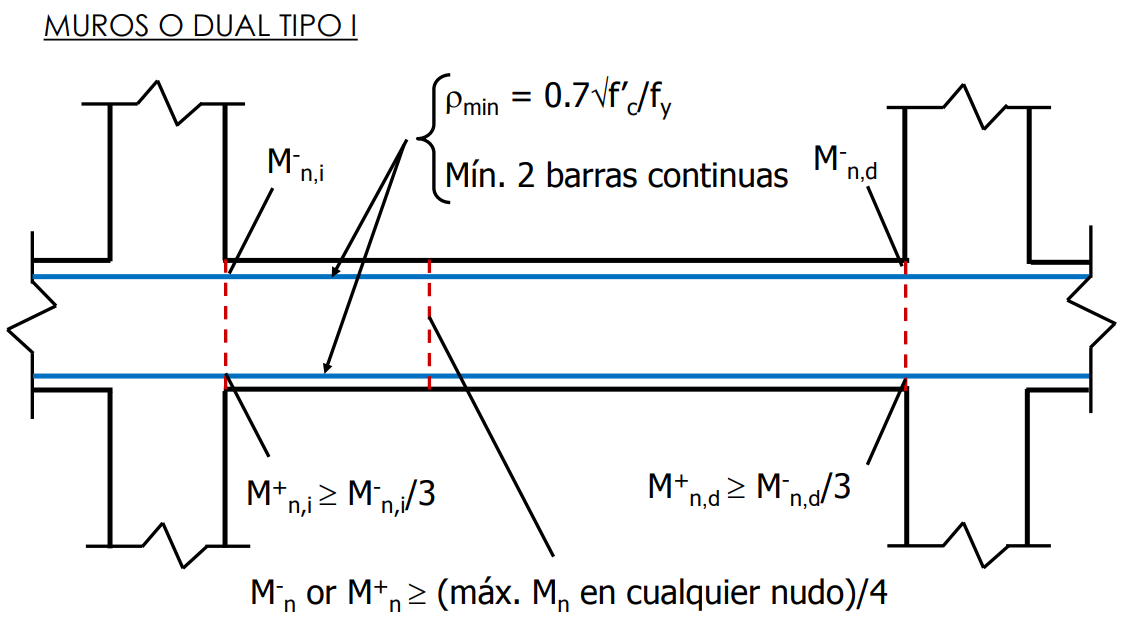
\includegraphics[width=90mm]{IMAGENES/d2.PNG}}\hspace{0mm}
    \subfigure[Sistemas de pórticos o duales]{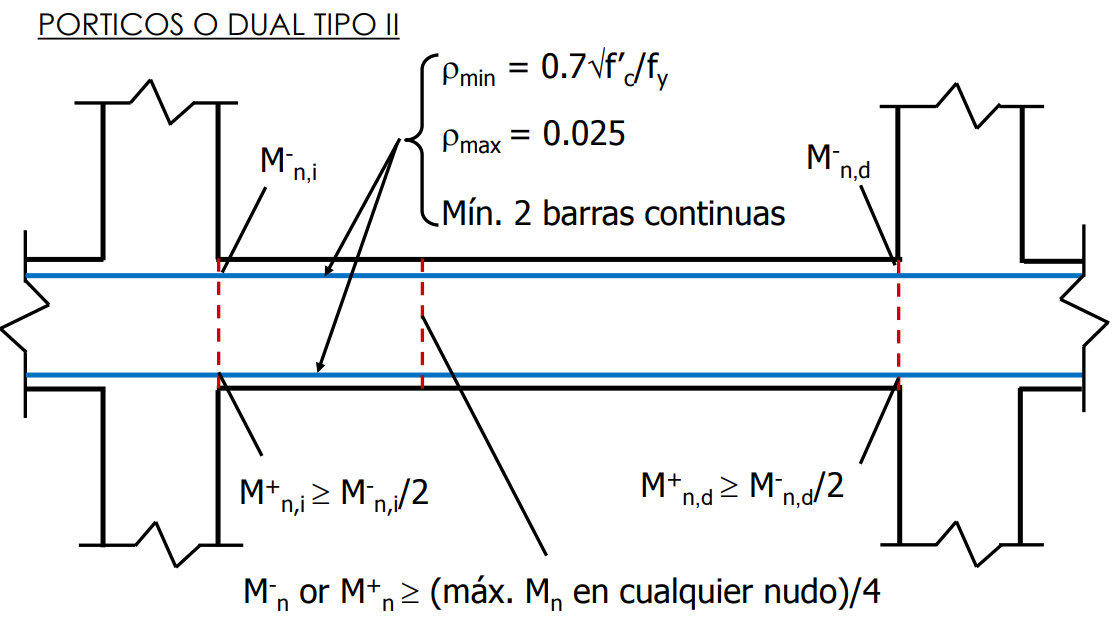
\includegraphics[width=90mm]{IMAGENES/d3.PNG}}
    \caption*{Fuente: \cite{CAPUCP}}
    \label{reqv}
\end{figure}

\noindent En la dirección X se trata de un sistema de muros por lo que se exige que la resistencia a momento mínima en un nudo sea por lo menos la tercera parte del máximo, tal condición se cumple dado que el momento $\phi M_{n,1}$ es mayor que el 50\% que $\phi M_{n,2}$.

\subsubsection{Diseño a corte por capacidad}
\begin{theo}[Art. 21.4.3 y 21.5.4.1:]{thm:ca1}
\textit{Vigas en sistemas de muros}\\
La cortante de diseño para vigas que resistan efectos sísmicos se calculara como la suma del cortante asociado con el desarrollo de los momentos nominales (Mn) del elemento en cada extremo restringido de la luz libre y el cortante isostático calculado para las cargas de gravedad tributarias amplificadas.\\
El cortante máximo obtenido de las combinaciones de carga de diseño de 9.2.3 con un factor de amplificación para los valores del sismo igual a 2,5.\\
\textit{Vigas en sistemas de pórticos o duales}\\
La fuerza cortante de diseño, Vu, de los elementos en flexión, deberá determinarse a partir de la suma de las fuerzas cortantes asociadas con el desarrollo de las resistencias probables en flexión (Mpr = 1,25 Mn) en los extremos de la luz libre del elemento y la fuerza cortante isostática calculada para las cargas de gravedad tributarias amplificadas.
\end{theo}
\begin{align}
V_{u}=\frac{M_{p, i s q}+M_{p, d e r}}{l_{n}} \pm W_{u} \cdot \frac{l_{n}}{2}
\end{align}
\noindent Calculo de la carga distribuida sobre la viga:
\FPset\plosa{0.3}
\FPset\alosa{3.2}
\FPset\wpt{0.1}
\FPset\wlosa{0.2}
\FPeval{\wviga}{round((\plosa+\wpt)*\alosa+2.4*\bv*\h/10000,2)}
\FPeval{\wvigav}{round((\wlosa)*\alosa,2)}
\FPeval{\wvigau}{round(1.25*(\wviga+\wvigav),2)}
\begin{itemize}
  \item Peso distribuido de la losa aligerada: $w_{\text {alig }}=\plosa \mathrm{~ton} / \mathrm{m}^{2}$
  \item Ancho tributario de la losa aligerada: $A_{t}=\alosa \mathrm{~m}$
  \item Sobrecarga muerta por piso terminado: $w_{p t}=\wpt \mathrm{~ton}/ \mathrm{m}^{2}$
  \item Carga viva sobre losas: $w_{sc}=\wlosa \mathrm{~ton}/\mathrm{m}^{2}$
\end{itemize}
\newpage
\noindent Carga muerta total distribuida sobre la viga:
\begin{center}
$W_{c m}=b \cdot h \cdot \gamma_{c}+\left(w_{a l i g}+w_{p t}\right) \cdot A_{t}=\wviga \text {~ton}/{m}$
\end{center}
\noindent Carga viva distribuida  sobre la viga:
\begin{center}
$W_{c v}=w_{sc} \cdot A_{t}=\wlosa\cdot\alosa=\wvigav \text {~ton}/{m}$
\end{center}
\noindent Carga ultima sobre la viga:
\begin{center}
$W_{u}=1,25 \cdot\left(W_{c m}+W_{c v}\right)=1,25 \cdot\left(\wviga+\wvigav\right)=\wvigau \text {~ton}/{m}$
\end{center}
%\newpage
\begin{figure}[h!]
    \centering
    \subfigure[Sistemas de muros]{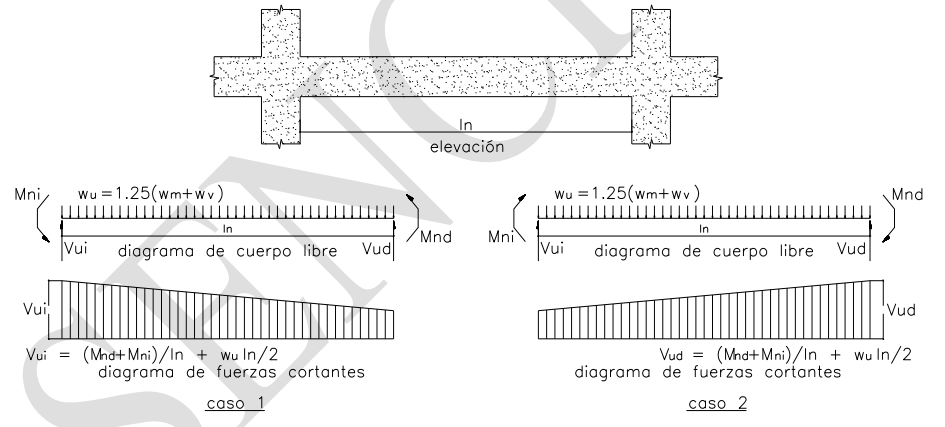
\includegraphics[width=130mm]{IMAGENES/d4.PNG}}\hspace{0mm}
    \subfigure[Sistemas de pórticos o duales]{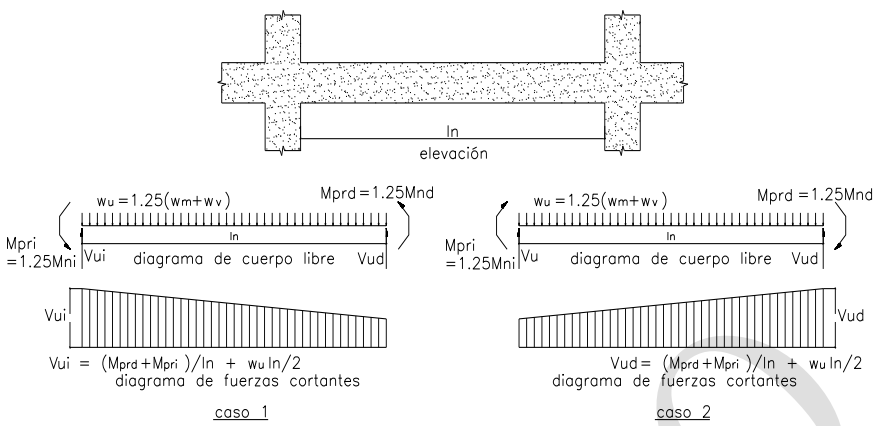
\includegraphics[width=130mm]{IMAGENES/d8.PNG}}
    \caption{Diseño por corte capacidad en vigas}
    \label{reqv}
\end{figure}
\FPeval{mncoru}{round(mncor/0.9,2)}
\FPeval{mnderu}{round(mnder/0.9,2)}
\newpage
\noindent CASO 1:\\
Momento negativo en el extremo izquierdo:
\begin{center}
$M_{n,isq-}=\mncor/0.9=\mncoru\;\mathrm{~ton.m}$
\end{center}
Momento positivo en el extremo derecho:
\begin{center}
$M_{n,der+}=M_{n,isq-}=\mncoru\;\mathrm{~ton.m}$
\end{center}
Cortante por capacidad:
\FPeval{\va}{round(2*\mncoru/\ln+\wvigau*\ln*0.5,2)}
\FPeval{\vb}{round(2*\mncoru/\ln-\wvigau*\ln*0.5,2)}
\begin{align*}
V_{1,1}&=\frac{2\cdot\mncoru}{\ln} + \wvigau  \cdot \frac{\ln}{2}=\va\text {~ton}\\
V_{1,2}&=\frac{2\cdot\mncoru}{\ln} - \wvigau  \cdot \frac{\ln}{2}=\vb\text {~ton}
\end{align*}
CASO 2:\\
\FPeval{\vc}{round((\mnderu+\mncoru)/\ln+\wvigau*\ln*0.5,2)}
\FPeval{\vd}{round((\mnderu+\mncoru)/\ln-\wvigau*\ln*0.5,2)}
Momento positivo en el extremo izquierdo: 
\begin{center}
$M_{n,isq-}=\mncor/0.9=\mncoru\;\mathrm{~ton.m}$
\end{center}
Momento negativo en el extremo derecho: 
\begin{center}
$\displaystyle M_{n,der+}=\mnder/0.9=\mnderu\;\mathrm{~ton.m}$
\end{center}
Cortante por capacidad:
\begin{align*}
V_{2,1}=\frac{\mncoru+\mnderu}{\ln} + \wvigau  \cdot \frac{\ln}{2}=\vc\text {~ton}\\
V_{2,2}=\frac{\mncoru+\mnderu}{\ln} - \wvigau  \cdot \frac{\ln}{2}=\vd\text {~ton}
\end{align*}
En la figura \ref{cor} se muestra las cortantes por capacidad y dado que se trata de una viga perteneciente a un sistema de muros también se muestra las cortantes máximas para las combinaciones de sismo con un factor de amplificación de 2,5 como se menciona en 21.4.3.
\newpage
\begin{figure}[h!]
    \centering
    \caption{Envolvente de cortantes}
    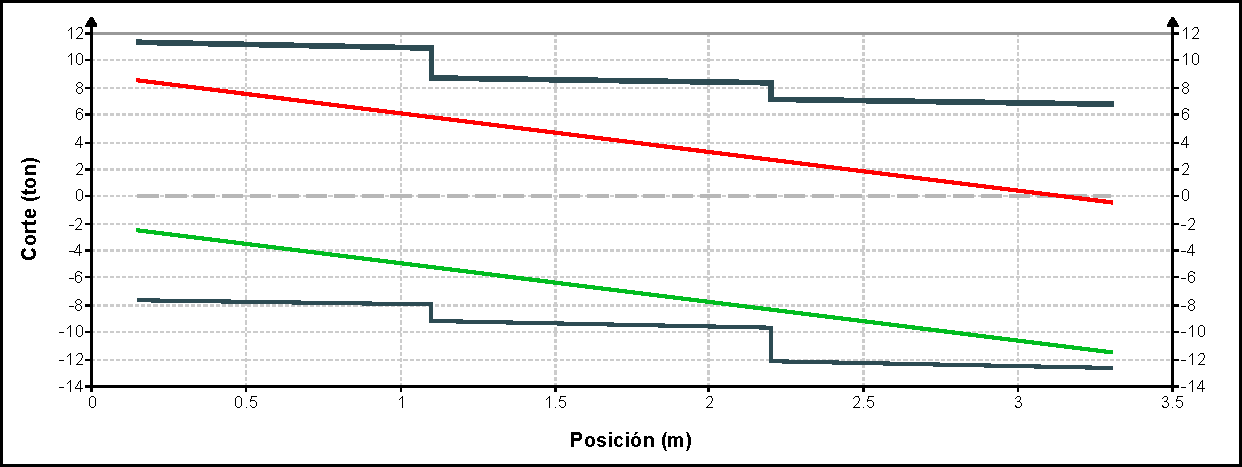
\includegraphics[scale=0.7]{IMAGENES/corta.pdf}
    %\caption*{\small Fuente: \it \cite{cordova2015}}
    \label{cor}
\end{figure}

\subsubsection{Disposiciones del refuerzo transversal en las zonas de confinamiento de vigas}
En ambos extremos del elemento deben disponerse estribos cerrados de confinamiento en longitudes iguales a dos veces el peralte del elemento medido desde la cara del elemento de apoyo hacia el centro de la luz, ya que en estas zonas puede ocurrir fluencia por flexión debido a desplazamientos laterales inelásticos de la estructura.
\begin{theo}[Art. 21.4.4.4 y 21.5.3.2 :]{thm:ca1}
\textit{Vigas en sistemas de muros}\\
El primer estribo cerrado de confinamiento debe estar situado a no más de 100 mm de la cara del elemento de apoyo.  Los estribos serán como mínimo de 8 mm de diámetro para barras longitudinales de hasta 5/8" de diámetro, de 3/8" para barras longitudinales de hasta  1" de diámetro y de 1/2" para barras longitudinales de mayor diámetro. \\
\textit{Vigas en sistemas de pórticos o duales}\\
Los estribos serán como mínimo de 3/8" para barras longitudinales de hasta 1" de diámetro y de  1/2"  para  barras  longitudinales  de  mayor  diámetro. El primer  estribo  cerrado  de confinamiento debe estar situado a no más de 50 mm de la cara del elemento de apoyo.
\end{theo}
\newpage
\noindent El espaciamiento del refuerzo transversal en vigas de sistemas de muros no debe exceder el menor de:
%\vspace{-0.3cm}
\begin{enumerate}
\item[] (a): $d / 4 \geq 15 \mathrm{~cm}$
\item[] (b): $10d_{b}$
\item[] (c): $24d_{e}$
\item[] (d): $30 \mathrm{~cm}$
\end{enumerate}
\noindent
Donde:\\
$d$: Peralte efectivo\\
$d_{b}$: Diámetro de la barra longitudinal de menor diámetro\\
$d_{e}$: Diámetro del estribo\\
En vigas de sistemas de pórticos o duales la condición (b) cambia por: $8d_{b}$ y se debe cumplir que en las zonas de confinamiento, la distancia horizontal entre las ramas verticales del refuerzo transversal (estribos cerrados y/o grapas suplementarias) no deberá exceder de 300 mm (Art. 21.5.3.3)\\
Para el presente caso se tiene:
\FPeval{\dcuar}{round(\defe/4,2)}
\FPeval{\conb}{round(\vacm*10,2)}
\FPeval{\conc}{round(\estcm*24,2)}
\FPeval{\lcon}{round(\h*2/100,2)}
\begin{enumerate}
\item[] (a): $d / 4=\dcuar\mathrm{~cm} \geq 15 \mathrm{~cm}$
\item[] (b): $10d_{b}=\conb\mathrm{~cm}$
\item[] (c): $24d_{e}=\conc\mathrm{~cm}$
\item[] (d): $30 \mathrm{~cm}$
\end{enumerate}
Por lo tanto la separación final de estribos dentro de la longitud de confinamiento $2h=\lcon\mathrm{~m}$ sera 10cm.
\newpage
\subsubsection{Disposiciones del refuerzo transversal fuera de la zona de confinamiento en vigas}
\begin{theo}[Art. 21.4.4.4 y 21.5.3.2 :]{thm:ca1}
\textit{Vigas en sistemas de muros}\\
Los estribos deben estar espaciados a no más de 0,5d a lo largo de la longitud del elemento. En todo el elemento la separación de los estribos, no deberá ser mayor que la requerida por fuerza cortante. \\
\textit{Vigas en sistemas de pórticos o duales}\\
Fuera  de  las  zonas  de  confinamiento,  deben  colocarse  estribos  cerrados con  ganchos sísmicos en ambos extremos, espaciados a no más de d/2 en toda la longitud del elemento. En todo el elemento la separación de los estribos, no será mayor que la requerida por fuerza cortante.
\end{theo}
\FPeval{\sepf}{round(\defe/2,2)}
\noindent La separación del refuerzo transversal fuera de la zona de confinamiento sera: $s=d/2=\sepf\approx20\mathrm{~cm}$\\
Por lo tanto, el diseño final a cortante de la viga será:
\begin{center}
$1 @ 5 \mathrm{~cm}, 10 @ 10 \mathrm{~cm}$, Rto.@20cm   
\end{center}
\subsubsection{Disposiciones adicionales para vigas en sistemas de pórticos o duales}
\begin{theo}[Art. 21.4.4.4 y 21.5.3.2 :]{thm:ca1}
Sólo se permiten empalmes por traslape del refuerzo de flexión cuando se proporcionan estribos de confinamiento o espirales en la toda longitud del empalme.   El espaciamiento del refuerzo transversal que envuelve las barras traslapadas no debe exceder el menor de d/4 ó 150 mm.
\end{theo}
\newpage
\noindent No deben emplearse empalmes por traslape:
\begin{enumerate}
\item[] (a): dentro los nudos
\item[] (b): en una distancia de dos veces el peralte del elemento medida desde la cara del nudo
\item[] (c): donde  el  análisis  indique  fluencia  por  flexión  del  refuerzo causada  por  los desplazamientos laterales inelásticos del pórtico.
\end{enumerate}
\begin{figure}[h!]
    \centering
      \caption{Resumen de requisitos del refuerzo transversal en vigas}
    \subfigure[Sistemas de muros]{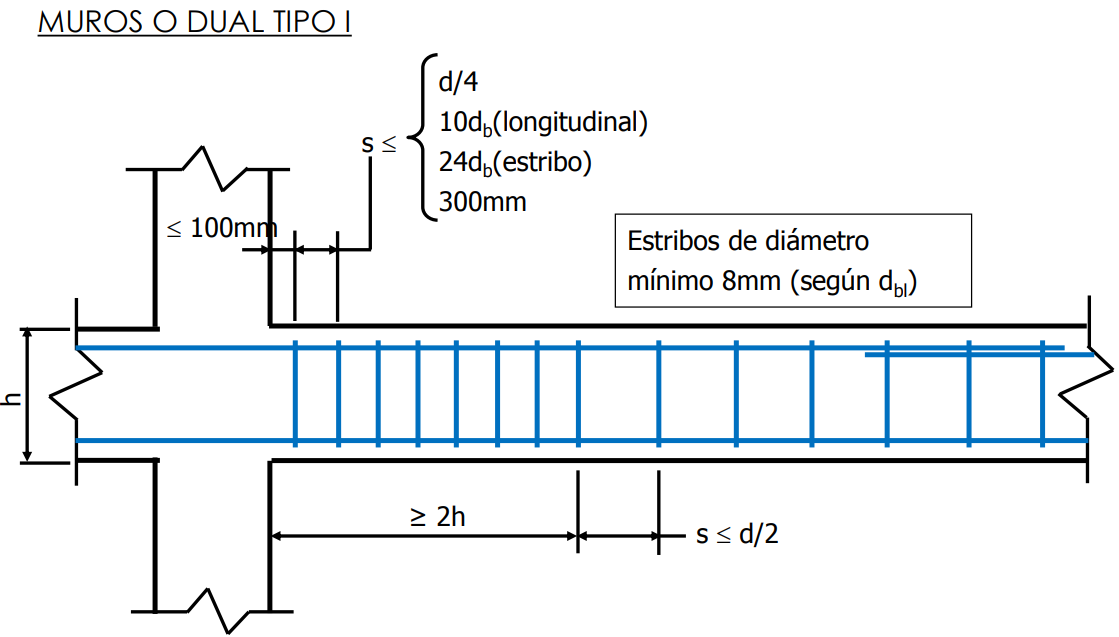
\includegraphics[width=95mm]{IMAGENES/d6.PNG}}\hspace{0mm}
    \subfigure[Sistemas de pórticos o duales]{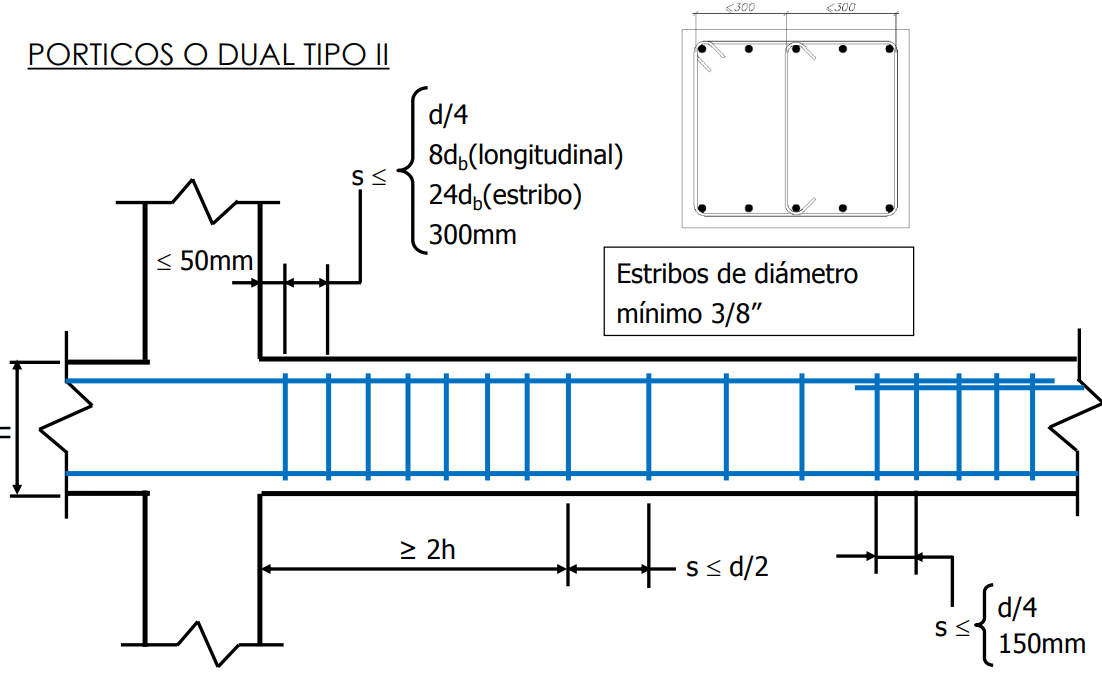
\includegraphics[width=95mm]{IMAGENES/d7.PNG}}
    \caption*{Fuente: \cite{CAPUCP}}
    \label{reqv}
\end{figure}
\subsubsection{Resistencia a corte Cap. 11}
La resistencia a cortante de la sección, concreto y acero transversal esta dado respectivamente por:
\begin{flalign}
&\textup{Ecu.(11.1) y (11.2) E-060:}&\phi V_{n}&=\phi_{c} \cdot\left(V_{c}+V_{e}\right)&&\\
&\textup{Ecu.(11.3) E-060:}&V_{c}&=0,53 \cdot \sqrt{f_{c}^{\prime}} \cdot b \cdot d&&\label{vc}\\
&\textup{Ecu.(11.15) E-060:}&V_{e}&=\frac{n \cdot A_{s h} \cdot f_{y} \cdot d}{s}&&\label{vmax}
\end{flalign}
\noindent
Donde:\\
$n$ : Numero de ramas de estribos\\
$A_{s h}:$ Área del acero transversal\\
$s:$ Separación del refuerzo transversal\\
La cortante máxima que pueden tomar los estribos esta dado por:
\begin{flalign}
&\textup{Art. 11.5.7.9 E-060:}&V_{e, \max }&=2,1 \cdot \sqrt{f_{c}^{\prime}} \cdot b \cdot d&&
\end{flalign}
\noindent
%Verificación de la capacidad a fuerza cortante de la viga:\\
Cortante resistente por el concreto según \ref{vc}:
\FPeval{\vcon}{round(0.53*\rc*\bv*\defe/1000,2)}
\begin{center}
$V_{c}=0,53 \cdot \sqrt{f_{c}^{\prime}} \cdot b \cdot d=0,53 \cdot \sqrt{\fc} \cdot \bv \cdot \defe=\vcon\mathrm{~ton}$
\end{center}
Cortante resistente por los estribos en la zona de confinamiento:
\FPeval{\ves}{round(2*0.71*\fy*\defe/10000,2)}
\begin{center}
$\displaystyle V_{e,1}=\frac{n \cdot A_{s h} \cdot f_{y} \cdot d}{s}=\frac{2 \cdot 0,71 \cdot 4200 \cdot \defe}{10}=\ves \mathrm{ton}$
\end{center}
Cortante resistente por los estribos fuera de la zona de confinamiento:
\FPeval{\vesf}{round(2*0.71*\fy*\defe/20000,2)}
\begin{center}
$\displaystyle V_{e,2}=\frac{n \cdot A_{s h} \cdot f_{y} \cdot d}{s}=\frac{2 \cdot 0,71 \cdot 4200 \cdot \defe}{20}=\vesf \mathrm{ton}$
\end{center}
Cortante máxima que pueden soportar los estribos:
\FPeval{\vmax}{round(2.1*\rc*\bv*\defe/1000,2)}
\begin{center}
$\displaystyle V_{e, \max }=2,1 \cdot \sqrt{\fc} \cdot \bv \cdot \defe=\vmax\mathrm{ton}>V_{e}=\ves\mathrm{ton}$ 
\end{center}
Cortante nominal en la zona de confinamiento:
\FPeval{\vnom}{round((\vcon+\ves)*0.85,2)}
\begin{center}
$\displaystyle \phi V_{n,1}=\phi_{c} \cdot\left(V_{c}+V_{e}\right)=0,85 \cdot(\vcon+\ves)=\vnom\mathrm{Ton}$
\end{center}
Cortante nominal fuera de la zona de confinamiento:
\FPeval{\vnomf}{round((\vcon+\vesf)*0.85,2)}
\begin{center}
$\displaystyle \phi V_{n,2}=\phi_{c} \cdot\left(V_{c}+V_{e}\right)=0,85 \cdot(\vcon+\vesf)=\vnomf\mathrm{ton}$
\end{center}
Según el artículo 11.1.3.1 se permite diseñar los elementos para la fuerza cortante a una distancia $d$ de la cara.\\
Como se aprecia en la figura \ref{corcap} al cumplir las disposiciones del refuerzo transversal se cumple holgadamente con las solicitaciones máximas de la viga a cortante.
\begin{figure}[h!]
    \centering
    \caption{Demanda capacidad a corte de la viga}
    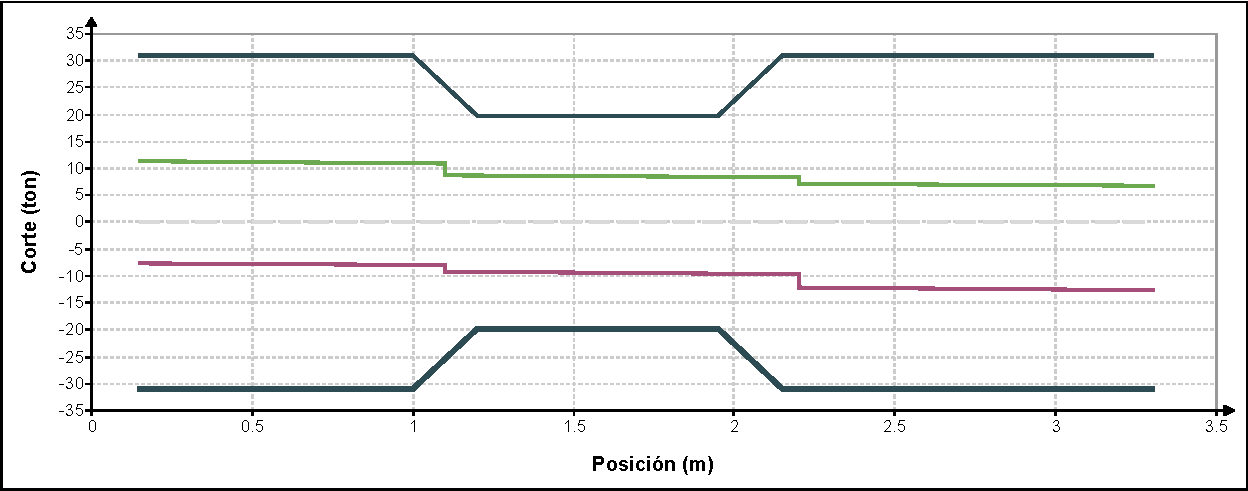
\includegraphics[scale=0.7]{IMAGENES/capcor.pdf}
    %\caption*{\small Fuente: \it \cite{cordova2015}}
    \label{corcap}
\end{figure}
